\documentclass{standalone}
\usepackage{tikz}
\usetikzlibrary{patterns, positioning}
\usepackage[sfdefault]{ClearSans} %% option 'sfdefault' activates Clear Sans as the default text font
\usepackage[T1]{fontenc}

\begin{document}
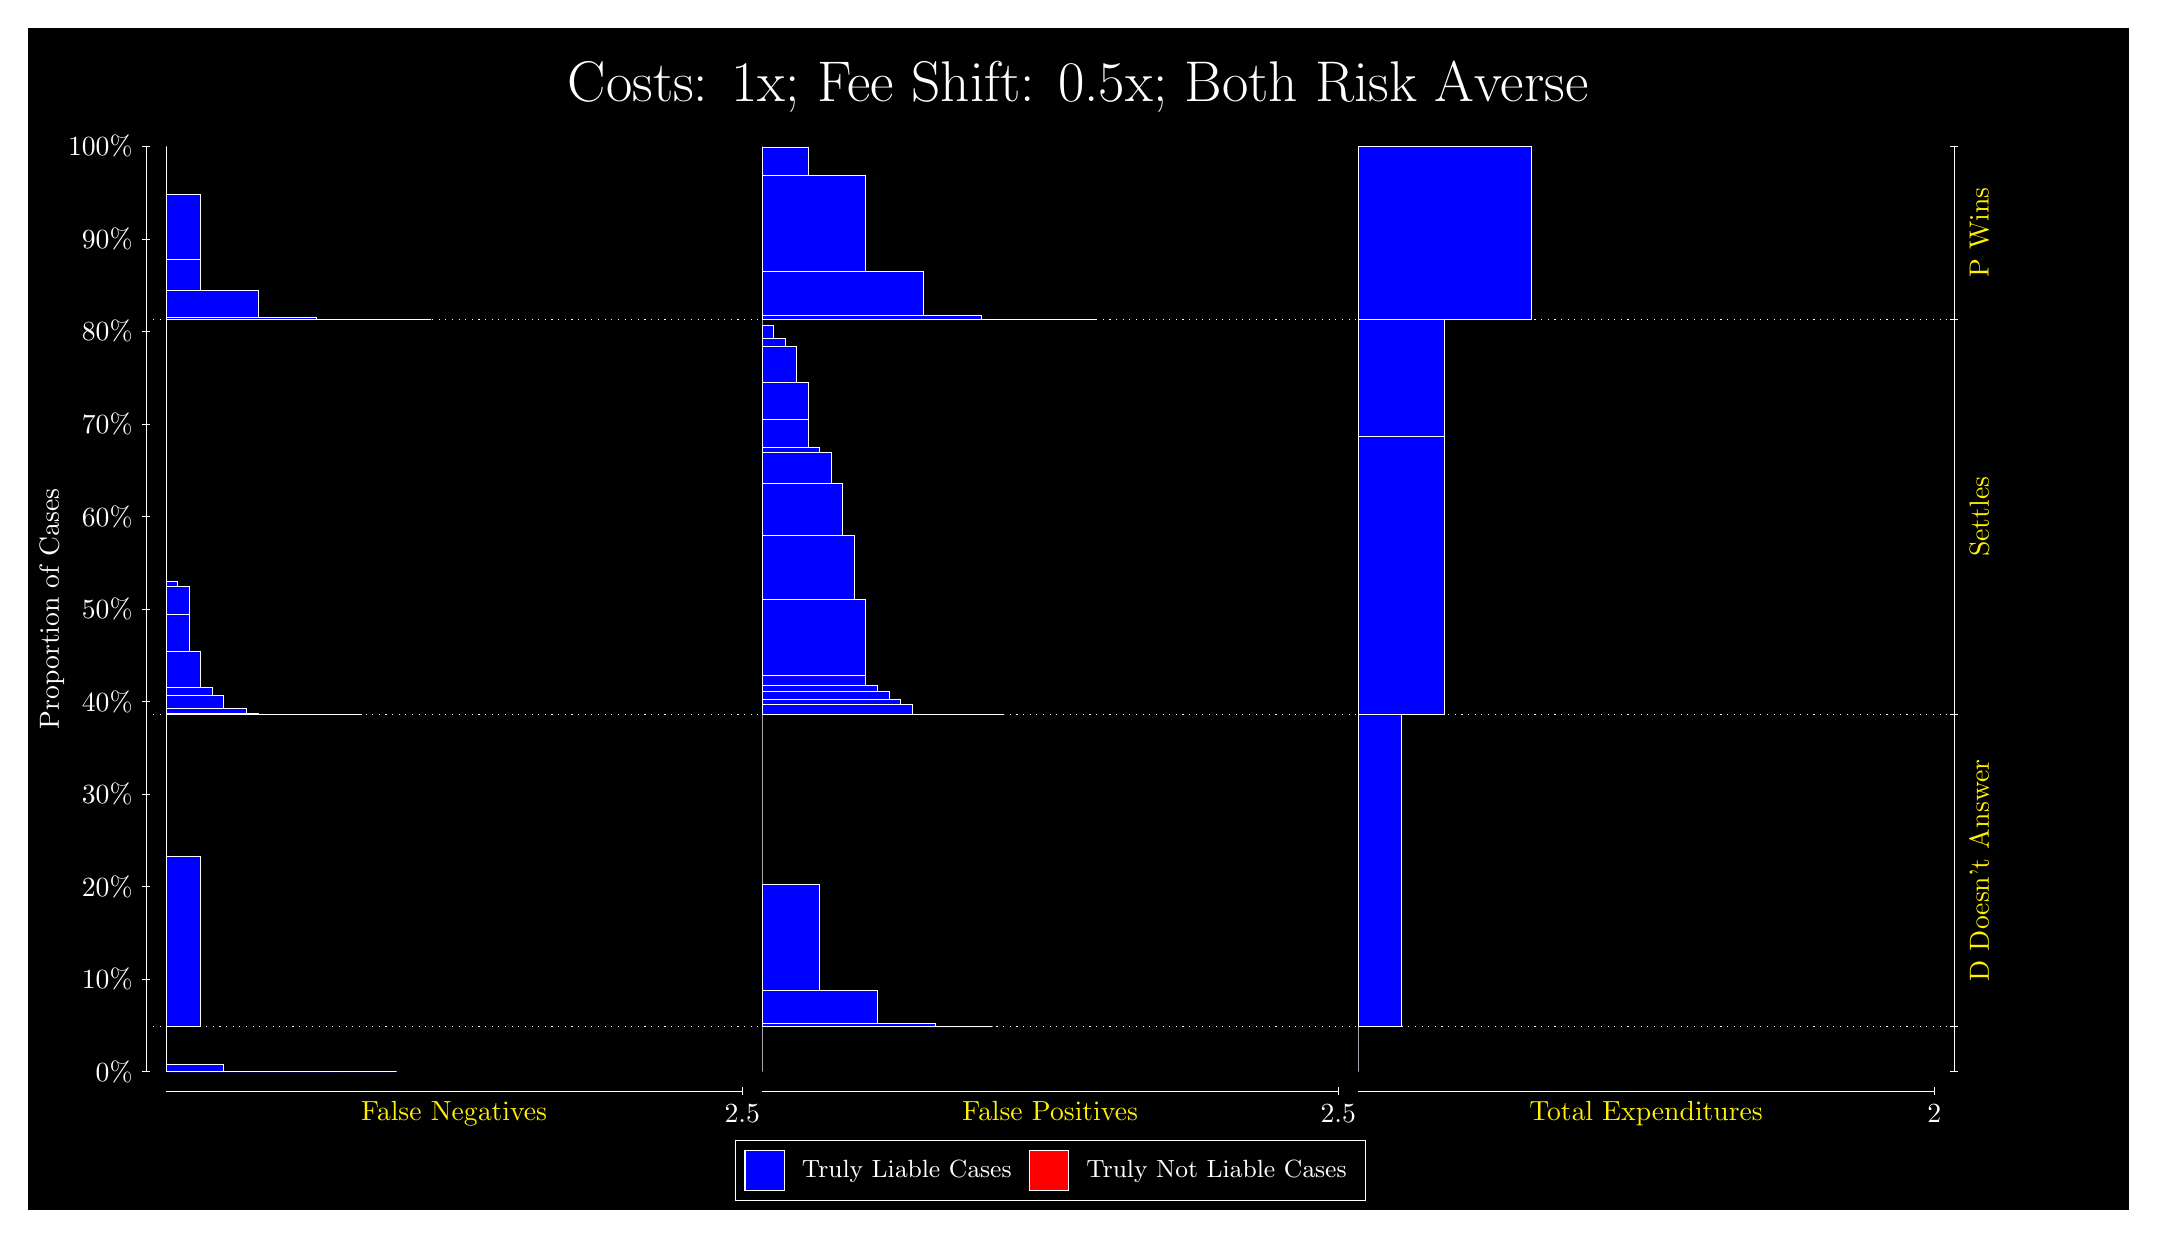
\begin{tikzpicture}
\draw[fill=black] (0,0) rectangle (26.667,15);
\draw[text=white] (0,13.5) rectangle (26.667,15) node[midway] {\huge Costs: 1x; Fee Shift: 0.5x; Both Risk Averse};
\draw[white, very thin] (1.5,1.75) -- (1.5,13.5);
\node[rotate=90, text=white, anchor=center] at (0.3, 7.625) {Proportion of Cases};
\draw[white, very thin] (1.45,1.75) -- (1.55,1.75);
\node[text=white, anchor=east] at (1.45, 1.75) {0\%};
\draw[white, very thin] (1.45,2.925) -- (1.55,2.925);
\node[text=white, anchor=east] at (1.45, 2.925) {10\%};
\draw[white, very thin] (1.45,4.1) -- (1.55,4.1);
\node[text=white, anchor=east] at (1.45, 4.1) {20\%};
\draw[white, very thin] (1.45,5.275) -- (1.55,5.275);
\node[text=white, anchor=east] at (1.45, 5.275) {30\%};
\draw[white, very thin] (1.45,6.45) -- (1.55,6.45);
\node[text=white, anchor=east] at (1.45, 6.45) {40\%};
\draw[white, very thin] (1.45,7.625) -- (1.55,7.625);
\node[text=white, anchor=east] at (1.45, 7.625) {50\%};
\draw[white, very thin] (1.45,8.8) -- (1.55,8.8);
\node[text=white, anchor=east] at (1.45, 8.8) {60\%};
\draw[white, very thin] (1.45,9.975) -- (1.55,9.975);
\node[text=white, anchor=east] at (1.45, 9.975) {70\%};
\draw[white, very thin] (1.45,11.15) -- (1.55,11.15);
\node[text=white, anchor=east] at (1.45, 11.15) {80\%};
\draw[white, very thin] (1.45,12.325) -- (1.55,12.325);
\node[text=white, anchor=east] at (1.45, 12.325) {90\%};
\draw[white, very thin] (1.45,13.5) -- (1.55,13.5);
\node[text=white, anchor=east] at (1.45, 13.5) {100\%};

\draw[white, very thin] (24.457,1.75) -- (24.457,13.5);
\draw[white, very thin] (24.407,1.75) -- (24.507,1.75);
\node[anchor=west] at (24.407, 1.75) {};
\draw[white, very thin] (24.407,2.3201) -- (24.507,2.3201);
\node[anchor=west] at (24.407, 2.3201) {};
\draw[white, very thin] (24.407,6.2858) -- (24.507,6.2858);
\node[anchor=west] at (24.407, 6.2858) {};
\draw[white, very thin] (24.407,11.306) -- (24.507,11.306);
\node[anchor=west] at (24.407, 11.306) {};
\draw[white, very thin] (24.407,13.5) -- (24.507,13.5);
\node[anchor=west] at (24.407, 13.5) {};

\draw[white, very thin, fill=blue] (1.75,1.75) rectangle (4.6775,1.75);
\draw[white, very thin, fill=blue] (1.75,1.75) rectangle (3.9457,1.75);
\draw[white, very thin, fill=blue] (1.75,1.75) rectangle (3.2138,1.7508);
\draw[white, very thin, fill=blue] (1.75,1.7508) rectangle (2.4819,1.8433);
\draw[white, very thin, fill=red] (1.75,1.8433) rectangle (1.75,1.8433);
\draw[white, very thin, fill=blue] (1.75,1.8433) rectangle (1.75,2.3201);
\draw[white, very thin, fill=blue] (1.75,2.3201) rectangle (2.1891,4.4816);
\draw[white, very thin, fill=red] (1.75,4.4816) rectangle (1.75,4.4816);
\draw[white, very thin, fill=blue] (1.75,4.4816) rectangle (1.75,6.2858);
\draw[white, very thin, fill=blue] (1.75,6.2858) rectangle (4.2384,6.2858);
\draw[white, very thin, fill=blue] (1.75,6.2858) rectangle (3.9457,6.2858);
\draw[white, very thin, fill=blue] (1.75,6.2858) rectangle (3.6529,6.2858);
\draw[white, very thin, fill=blue] (1.75,6.2858) rectangle (3.5065,6.2859);
\draw[white, very thin, fill=blue] (1.75,6.2859) rectangle (3.3602,6.2859);
\draw[white, very thin, fill=blue] (1.75,6.2859) rectangle (3.2138,6.2859);
\draw[white, very thin, fill=blue] (1.75,6.2859) rectangle (3.0674,6.2861);
\draw[white, very thin, fill=blue] (1.75,6.2861) rectangle (2.921,6.3009);
\draw[white, very thin, fill=blue] (1.75,6.3009) rectangle (2.7746,6.366);
\draw[white, very thin, fill=blue] (1.75,6.366) rectangle (2.6283,6.3664);
\draw[white, very thin, fill=blue] (1.75,6.3664) rectangle (2.4819,6.5334);
\draw[white, very thin, fill=blue] (1.75,6.5334) rectangle (2.3355,6.6295);
\draw[white, very thin, fill=blue] (1.75,6.6295) rectangle (2.1891,7.091);
\draw[white, very thin, fill=blue] (1.75,7.091) rectangle (2.0428,7.5602);
\draw[white, very thin, fill=blue] (1.75,7.5602) rectangle (2.0428,7.9099);
\draw[white, very thin, fill=blue] (1.75,7.9099) rectangle (1.8964,7.9795);
\draw[white, very thin, fill=red] (1.75,7.9795) rectangle (1.75,7.9795);
\draw[white, very thin, fill=blue] (1.75,7.9795) rectangle (1.75,11.306);
\draw[white, very thin, fill=blue] (1.75,11.306) rectangle (5.1167,11.306);
\draw[white, very thin, fill=blue] (1.75,11.306) rectangle (4.3848,11.306);
\draw[white, very thin, fill=blue] (1.75,11.306) rectangle (3.6529,11.324);
\draw[white, very thin, fill=blue] (1.75,11.324) rectangle (2.921,11.677);
\draw[white, very thin, fill=blue] (1.75,11.677) rectangle (2.1891,12.066);
\draw[white, very thin, fill=blue] (1.75,12.066) rectangle (2.1891,12.889);
\draw[white, very thin, fill=red] (1.75,12.889) rectangle (1.75,12.889);
\draw[white, very thin, fill=blue] (1.75,12.889) rectangle (1.75,13.5);
\draw[white, very thin, fill=red] (9.3189,1.75) rectangle (9.3189,1.75);
\draw[white, very thin, fill=blue] (9.3189,1.75) rectangle (9.3189,2.3201);
\draw[white, very thin, fill=red] (9.3189,2.3201) rectangle (12.246,2.3201);
\draw[white, very thin, fill=blue] (9.3189,2.3201) rectangle (12.246,2.3201);
\draw[white, very thin, fill=blue] (9.3189,2.3201) rectangle (11.515,2.3609);
\draw[white, very thin, fill=blue] (9.3189,2.3609) rectangle (10.783,2.7782);
\draw[white, very thin, fill=blue] (9.3189,2.7782) rectangle (10.051,4.1243);
\draw[white, very thin, fill=blue] (9.3189,4.1243) rectangle (9.3189,6.2858);
\draw[white, very thin, fill=red] (9.3189,6.2858) rectangle (12.393,6.2858);
\draw[white, very thin, fill=blue] (9.3189,6.2858) rectangle (12.393,6.2858);
\draw[white, very thin, fill=red] (9.3189,6.2858) rectangle (12.1,6.2858);
\draw[white, very thin, fill=blue] (9.3189,6.2858) rectangle (12.1,6.2858);
\draw[white, very thin, fill=red] (9.3189,6.2858) rectangle (11.807,6.2858);
\draw[white, very thin, fill=blue] (9.3189,6.2858) rectangle (11.807,6.2859);
\draw[white, very thin, fill=blue] (9.3189,6.2859) rectangle (11.661,6.2859);
\draw[white, very thin, fill=red] (9.3189,6.2859) rectangle (11.515,6.2859);
\draw[white, very thin, fill=blue] (9.3189,6.2859) rectangle (11.515,6.2864);
\draw[white, very thin, fill=blue] (9.3189,6.2864) rectangle (11.368,6.2869);
\draw[white, very thin, fill=red] (9.3189,6.2869) rectangle (11.222,6.2869);
\draw[white, very thin, fill=blue] (9.3189,6.2869) rectangle (11.222,6.4187);
\draw[white, very thin, fill=blue] (9.3189,6.4187) rectangle (11.075,6.4801);
\draw[white, very thin, fill=red] (9.3189,6.4801) rectangle (10.929,6.4801);
\draw[white, very thin, fill=blue] (9.3189,6.4801) rectangle (10.929,6.5815);
\draw[white, very thin, fill=blue] (9.3189,6.5815) rectangle (10.783,6.6524);
\draw[white, very thin, fill=blue] (9.3189,6.6524) rectangle (10.636,6.7777);
\draw[white, very thin, fill=red] (9.3189,6.7777) rectangle (10.636,6.7777);
\draw[white, very thin, fill=blue] (9.3189,6.7777) rectangle (10.636,7.7506);
\draw[white, very thin, fill=blue] (9.3189,7.7506) rectangle (10.49,8.5576);
\draw[white, very thin, fill=blue] (9.3189,8.5576) rectangle (10.344,9.2153);
\draw[white, very thin, fill=blue] (9.3189,9.2153) rectangle (10.197,9.6123);
\draw[white, very thin, fill=blue] (9.3189,9.6123) rectangle (10.051,9.6819);
\draw[white, very thin, fill=blue] (9.3189,9.6819) rectangle (9.9044,10.032);
\draw[white, very thin, fill=blue] (9.3189,10.032) rectangle (9.9044,10.501);
\draw[white, very thin, fill=blue] (9.3189,10.501) rectangle (9.758,10.962);
\draw[white, very thin, fill=blue] (9.3189,10.962) rectangle (9.6116,11.058);
\draw[white, very thin, fill=blue] (9.3189,11.058) rectangle (9.4652,11.225);
\draw[white, very thin, fill=blue] (9.3189,11.225) rectangle (9.3189,11.306);
\draw[white, very thin, fill=red] (9.3189,11.306) rectangle (13.564,11.306);
\draw[white, very thin, fill=blue] (9.3189,11.306) rectangle (13.564,11.306);
\draw[white, very thin, fill=red] (9.3189,11.306) rectangle (12.832,11.306);
\draw[white, very thin, fill=blue] (9.3189,11.306) rectangle (12.832,11.307);
\draw[white, very thin, fill=red] (9.3189,11.307) rectangle (12.1,11.307);
\draw[white, very thin, fill=blue] (9.3189,11.307) rectangle (12.1,11.356);
\draw[white, very thin, fill=red] (9.3189,11.356) rectangle (11.368,11.356);
\draw[white, very thin, fill=blue] (9.3189,11.356) rectangle (11.368,11.917);
\draw[white, very thin, fill=red] (9.3189,11.917) rectangle (10.636,11.917);
\draw[white, very thin, fill=blue] (9.3189,11.917) rectangle (10.636,13.129);
\draw[white, very thin, fill=blue] (9.3189,13.129) rectangle (9.9044,13.482);
\draw[white, very thin, fill=blue] (9.3189,13.482) rectangle (9.3189,13.5);
\draw[white, very thin, fill=red] (16.888,1.75) rectangle (16.888,1.75);
\draw[white, very thin, fill=blue] (16.888,1.75) rectangle (16.888,2.3201);
\draw[white, very thin, fill=red] (16.888,2.3201) rectangle (17.437,2.3201);
\draw[white, very thin, fill=blue] (16.888,2.3201) rectangle (17.437,6.2858);
\draw[white, very thin, fill=red] (16.888,6.2858) rectangle (17.986,6.2858);
\draw[white, very thin, fill=blue] (16.888,6.2858) rectangle (17.986,9.8172);
\draw[white, very thin, fill=red] (16.888,9.8172) rectangle (17.986,9.8172);
\draw[white, very thin, fill=blue] (16.888,9.8172) rectangle (17.986,11.306);
\draw[white, very thin, fill=red] (16.888,11.306) rectangle (19.083,11.306);
\draw[white, very thin, fill=blue] (16.888,11.306) rectangle (19.083,13.5);
\draw[white, dotted] (1.5,2.3201) -- (24.457,2.3201);
\draw[white, dotted] (1.5,6.2858) -- (24.457,6.2858);
\draw[white, dotted] (1.5,11.306) -- (24.457,11.306);
\draw[white, very thin] (1.75,1.5) -- (9.0689,1.5);
\node[text=yellow, anchor=north] at (5.4094, 1.5) {False Negatives};
\draw[white, very thin] (9.0689,1.45) -- (9.0689,1.55);
\node[text=white, anchor=north] at (9.0689, 1.45) {2.5};

\draw[white, very thin] (9.3189,1.5) -- (16.638,1.5);
\node[text=yellow, anchor=north] at (12.978, 1.5) {False Positives};
\draw[white, very thin] (16.638,1.45) -- (16.638,1.55);
\node[text=white, anchor=north] at (16.638, 1.45) {2.5};

\draw[white, very thin] (16.888,1.5) -- (24.207,1.5);
\node[text=yellow, anchor=north] at (20.547, 1.5) {Total Expenditures};
\draw[white, very thin] (24.207,1.45) -- (24.207,1.55);
\node[text=white, anchor=north] at (24.207, 1.45) {2};


\node[text=yellow, centered, rotate=90] at (24.777, 4.3029) {D Doesn't Answer};
\node[text=yellow, centered, rotate=90] at (24.777, 8.7959) {Settles};
\node[text=yellow, centered, rotate=90] at (24.777, 12.403) {P Wins};

\draw (12.978300999999998,1.5) node[draw=none] (baseCoordinate) {};
\begin{scope}[align=center]
        \matrix[scale=0.5, draw=white, below=0.5cm of baseCoordinate, nodes={draw}, column sep=0.1cm]{
            \node[rectangle, draw, minimum width=0.5cm, minimum height=0.5cm, fill=blue] {}; &
            \node[draw=none, font=\small, text=white] (B) {Truly Liable Cases}; &
            \node[rectangle, draw, minimum width=0.5cm, minimum height=0.5cm, fill=red] {}; &
            \node[draw=none, font=\small, text=white] (B) {Truly Not Liable Cases}; \\
            };
\end{scope}

\end{tikzpicture}
\end{document}